\newpage
\thispagestyle{plain}
\section{Least-Squares-Support Vector Machine}

In diesem Abschnitt soll das Bayesian Framework auf ein bekanntes Problem angewendet werden, genauer die Klassifizierung von Daten. Es wird dabei im folgenden die Binärklassifizierung betrachtet.\\
Generell ist bei solchen Problemen immer ein Datensatz \((x_i,y_i)_{i=1,\dots,n}\) von Features \(x_i\in\mathbb{R}^{n_f}\) und Klassenzugehörigkeiten \(y_i=\pm1\) gegeben. Diese Daten werden auch Trainingsobjekte genannt. Jedes Objekt wird durch einen Vektor \(x_i\) in einem Vektorraum repräsentiert. Aufgabe der Support Vector Machine ist es nun, in diesen Raum eine Hyperebene zu finden, die als Trennfläche dient und die Trainingsobjekte in zwei Klassen teilt. Der Abstand der Vektoren, die der Hyperebene am nächsten liegen, wird dabei maximiert. Dieser breite, leere Rand soll später dafür sorgen, dass auch Objekte, die nicht genau den Trainingsobjekten entsprechen, möglichst zuverlässig klassifiziert werden.\\[0,5cm]
Beim Einsetzen der Hyperebene ist es nicht notwendig, alle Trainingsvektoren zu beachten. Vektoren, die weiter von der Hyperebene entfernt liegen, beeinflussen Lage und Position der Trennebene nicht. Die Hyperebene ist nur von den ihr am nächsten liegenden Vektoren abhängig, und auch nur diese werden benötigt, um die Ebene mathematisch exakt zu beschreiben. Diese nächstliegenden Vektoren werden nach ihrer Funktion Stützvektoren (engl. support vectors) wodurch sich der Name Support Vector Machines (SVM) erklärt. \\[0,5cm]
Weiterhin ist es wichtig zu beachten, dass eine Hyperebene nicht verbogen werden kann, weshalb die Daten zur Nutzung einer linearen Trennebene auch linear separierbar sein müssen. Da dies aber in der Realität nicht häufig der Fall ist, werden im Nachfolgenden die beiden Fälle der linear und nicht-linear trennbaren Trainingsdaten betrachtet.

\subsection{Klassische Support Vector Machine}

\subsubsection{Linear trennbare Daten}

\begin{defi}[Hyperebene]
	Eine Hyperebene im \(n\)-dimensionalen euklidischen Raum \(\mathbb{R}^n\) ist eine Teilmenge \(H\in\mathbb{R}\) der Form
	\begin{align*}
		H\;=\;\lbrace x\in\mathbb{R}^n\:|\:w^Tx+b\;=\;0\rbrace,
	\end{align*}
	wobei \(w\in\mathbb{R}^n\setminus\lbrace0\rbrace\) ein Normalenvektor der Hyperebene ist. Die Variable \(b\) wird hierbei \textit{Bias} genannt.
\end{defi}

Sind zwei Klassen von Beispielen durch eine Hyperebene voneinander linear trennbar, gibt es in der Regel unendlich viele Hyperebenen, welche beide Klassen voneinander trennen. Die SVM versucht nun, von allen möglichen trennenden Hyperebenen diejenige mit minimaler quadratischer Norm \(\|w\|^2_2\) auszuwählen, so dass gleichzeitig \(y_i\left(w^Tx_i+b\right)\geq 1\) für jedes Trainingsbeispiel \(x_i\) gilt. Dies ist äquivalent zur Maximierung des kleinsten Abstands zur Hyperebene, dem sogenannten Margin. Da hierbei keine Fehler in der Trennung zugelassen werden müssen, spricht man vor allem im Bezug zu nicht-linear trennbaren Daten auch von einem Hard-Margin. Insgesamt ergibt sich daraus der folgende Satz.

\begin{satz}[Primales SVM-Problem]
	Unter den obigen Vorüberlegungen definiert die Lösung des Minimierungsproblems
	\begin{align*}
		&\min_{w,b} \frac{1}{2}\|w\|^2_2\\
		&\text{unter } y_i\left(w^Tx_i+b\right)\geq 1
	\end{align*}
	diejenige Hyperebene, welche den Datensatz \((x_i,y_i)_{i=1,\dots,n}\) mit größtmöglichem Margin trennt. Für die namensgebenden Support Vektoren gilt hierbei Gleichheit in der Nebenbedingung. 
\end{satz}

\begin{proof}
	Siehe \cite{SVM}.
\end{proof}

Das oben beschriebene Optimierungsproblem wird normalerweise in seiner dualen Form gelöst. Diese Formulierung ist äquivalent zu dem primalen Problem, in dem Sinne, dass alle Lösungen des dualen auch Lösungen des primalen Problems sind. Die Umrechnung ergibt sich dadurch, dass der Normalenvektor \(w\) als Linearkombination von Trainingsdaten geschrieben werden kann:

\begin{align*}
	w\;=\;\sum_{i=1}^{n}\lambda_i y_i x_i
\end{align*}
Die duale Form wird mit Hilfe der Lagrange-Multiplikatoren und der Karush-Kuhn-Tucker-Bedingungen hergeleitet.

\begin{satz}[Duales SVM-Problem]
	Das primale SVM-Problem ist äquivalent zum dualen Minimierungsproblem
	\begin{align*}
		&\min_{\lambda} \frac{1}{2}\sum_{i=1}^{n}\sum_{j=1}^{n}\lambda_i\lambda_jy_iy_jx_i^Tx_j-\sum_{i=1}^{n}\lambda_i\\
		&\text{unter } \sum_{i=1}^{n}\lambda_iy_i\;=\;0,\\
		&\qquad\qquad\quad\:\:\: 0\leq\lambda_i.
	\end{align*}
\end{satz}

\begin{proof}
	Siehe \cite{SVM}.
\end{proof}

\begin{defi}[Entscheidungsfunktion]
	Um für konkrete Daten anhand der Lösung des vorherigen Minimierungsproblems entscheiden zu können, welcher Gruppe diese angehören, verwendet man die sogenannte \textit{Entscheidungsfunktion}
	\begin{align*}
		y\;=\;f(x)\;=\;\text{sign}\left(w^Tx+b\right).
	\end{align*}
	\label{defi:decision}
\end{defi}
Je nachdem, wo sich die Datenpunkte relativ zur Hyperebene befinden (also oberhalb oder unterhalb), ergibt die Anwendung der Hyperebenengleichung einen positiven oder negativen Wert, wobei nach Anwendung der Vorzeichenfunktion nur noch \(\pm1\) bleibt. Für Objekte, die genau auf der Trennebene liegen, wird der Wert zu \(0\).

\subsubsection{Nicht-linear trennbare Daten}

Um dem Problem der Nicht-linearen Trennbarkeit beizukommen, werden Schlupfvariablen \(e_i\) für jeden Datenpunkt \(x_i\) eingeführt. Diese sollen Fehler in der Nebenbedingung ausgleichen, wodurch Punkte im Margin selbst und sogar auf der falschen Seite der Hyperebene liegen können. Da die Verletzungen der Nebenbedingung möglichst klein gehalten werden sollen, werden die Schlupfvariablen in das Minimierungsproblem aufgenommen.

\begin{satz}[Primales SVM-Problem mit Soft-Margin]
	Unter den bei Soft Margin zulässigen Fehlern in der Trennung definiert die Lösung des Minimierungsproblems
	\begin{align*}
		 &\min_{w,b} \frac{1}{2}\|w\|^2_2 + \xi\sum_{i=1}^{n}e_i\\
		 &\text{unter } y_i\left(w^Tx_i+b\right)\geq 1-e_i,\\
		 &\qquad\qquad\qquad\quad\:\:\:\:  0\leq e_i,\\
		 &\qquad\qquad\qquad\quad\:\:\:\:  0< \xi
	\end{align*}
	diejenige Hyperebene, welche den Datensatz \((x_i,y_i)_{i=1,\dots,n}\) unter Zulässigkeit von Fehlern mit größtmöglichem Margin trennt.
\end{satz}

\begin{proof}
	Siehe \cite{SVM}.
\end{proof}

\begin{bem}
	Für die Support Vektoren gilt Gleichheit in der Nebenbedingung und \(e_i=0\). Für Datenpunkte, die innerhalb des Margin liegen, gilt \(e_i>0\) und Gleichheit in der Nebenbedingung.
\end{bem}

Wie schon beim linear-trennbaren Datensatz wird das Minimierungsproblem in seiner dualen Form gelöst.

\begin{satz}[Duales SVM-Problem mit Soft-Margin]
	Das primale SVM-Problem mit Soft Margin ist äquivalent zum dualen Minimierungsproblem
	\begin{align*}
		&\min_{\lambda} \frac{1}{2}\sum_{i=1}^{n}\sum_{j=1}^{n}\lambda_i\lambda_jy_iy_jx_i^Tx_j-\sum_{i=1}^{n}\lambda_i\\
		&\text{unter } \sum_{i=1}^{n}\lambda_iy_i\;=\;0,\\
		&\qquad\quad\:\:\: 0\leq\lambda_i\leq\xi.
	\end{align*}
\end{satz}

\begin{proof}
	Siehe \cite{SVM}.
\end{proof}

\subsubsection{Nicht-lineare Erweiterung mit Kernelfunktionen}

Die zuvor behandelten Darstellungen der SVM klassifizieren die Daten mittels einer linearen Funktion. Diese ist jedoch nur optimal, wenn auch das zu Grunde liegende Klassifikationsproblem linear ist. In vielen Anwendungen ist dies aber nicht der Fall. Ein möglicher Ausweg ist, die Daten in einen Raum höherer Dimension abzubilden. SVMs zeichnen sich dadurch aus, dass sich diese Erweiterung elegant einbauen lässt. Dazu benutzt man Transformationsfunktionen der Form
\begin{align*}
	\varphi \colon \mathbb {R} ^{d_{1}}\rightarrow \mathbb {R} ^{d_{2}},\quad x \mapsto \varphi (x).
\end{align*}
Dabei gilt \(d^1<d^2\), was die Anzahl möglicher trennender Abbildungen erhöht. Die Funktion \(\varphi\) ist allerdings aufwändig zu bestimmen, weshalb man den sogenannten \textit{Kernel-Trick} verwendet. In der dualen Formulierungen des Optimierungsproblems gehen die Datenpunkte \(x_i\) nur in Skalarprodukten ein. Um den Rechenaufwand zu reduzieren ersetzt man daher \(x_i^Tx_j\) durch \(\varphi(x_i)\varphi(x_j)\) und verwendet eine positiv definite \textit{Kernelfunktion}
\begin{align*}
	K(x_{i},x_{j})=\varphi (x_{i})^T\varphi (x_{j}).
\end{align*}
Dadurch kann eine Hyperebene in einem hochdimensionalen Raum implizit berechnet werden. Die Entscheidungsfunktion ergibt sich dabei direkt zu
\begin{align*}
	y\;=\;f(x)&\;=\;\text{sign}\left(\sum_{k=1}^{n}\lambda_ky_k\varphi(x_k)^T\varphi(x)+b\right)\\
	&\;=\;\text{sign}\left(\sum_{k=1}^{n}\lambda_ky_kK\left(x_k,x\right)+b\right),
\end{align*}
wenn man in Definition \autoref{defi:decision} mit \(w=\underset{k=1}{\overset{n}{\sum}}\lambda_ky_k\varphi(x_k)\) substituiert.\\[0,3cm]

Geeignete Kernelfunktionen sind zum Beispiel:
\begin{alignat*}{2}
	K(x,y)&\;=\;x^Ty && (\text{linear})\\
	K(x,y)&\;=\;\left(x^Ty+c\right)^d && (\text{polynomial})\\
	K(x,y)&\;=\;\exp \left(-{\tfrac {||x-y||^{{2}}}{2\sigma ^{{2}}}}\right) \qquad&& (\text{radial basis function, RBF})
\end{alignat*}

Andere Kernelfunktionen und weiterführende Untersuchungen sind zu finden in \cite{Kernel}.

\subsection{Least-Squares-SVM}

Wie zu Anfang des Kapitels erwähnt soll nun eine SVM mit Bayes-Framework hergeleitet werden. Dazu betrachtet man die Entscheidungsfunktion in allgemeiner Darstellung mit Kernelfunktion als Modellfunktion. Hierbei sind \(w\) und \(b\) Modellparameter, für welche nun a priori Verteilungsannahmen gemacht werden, um den MAP-Schätzer nach Proposition \autoref{prop:map} bestimmen zu können. Zusätzlich wird ein Parameter \(e\) eingeführt, welcher nun die Abweichung der Datenpunkte von der Hyperebene bzw. vom Rand des Margin darstellt. Die Annahmen an \(w\), \(b\) und die Abweichungen \(e_i\) lauten konkret:
\begin{enumerate}[(i)]
	\item \(w\) ist multivariat normalverteilt mit \(w\sim\mathcal{N}\left(0,\frac{1}{\mu}I_{n}\right)\).
	\item \(b\) ist normalverteilt mit \(b\sim\mathcal{N}\left(0,\sigma_b^2\right)\) und es gilt \(\sigma_b^2\rightarrow\infty\). Damit ist \(b\) im Grenzfall unbeschränkt gleichverteilt.
	\item \(w\) und \(b\) sind stochastisch unabhängig.
	\item Die Abweichungen \(e_i=1-y_i\left(w^T\varphi\left(x_i\right)+b\right)\) sind normalverteilt mit \(e_i\sim\mathcal{N}\left(0,\frac{1}{\xi}\right)\) und i.i.d.
	\item Der Datensatz \(D\) ist i.i.d.
\end{enumerate}
Die Annahme (i) erfolgt dabei aus ähnlichen Überlegungen, wie bei der Ridge Regression (Kapitel 2). Die Koeffizienten von \(w\) sollen demnach nicht zu groß werden, aber auch für den Prior ergeben sich Vereinfachungen durch die Normalverteilung.
Voraussetzung (ii) stellt dar, dass für \(b\) eine uniforme Annahme über die Verteilung gemacht wird, also keine Vorinformation in den Prior einfließen soll. Da eine herkömmliche Gleichverteilung jedoch beschränkt ist, verwendet man diesen Zugang.\\
Annahmen (iii) und (v) dienen zur Vereinfachung der a priori Verteilungen und ermöglichen erst deren Berechnung (s. u.). Die Forderung (iv) legt die Fehler \(e_i\) als Normalverteilt fest, aus ähnlichen Gründen wie bei (i). Durch die Gleichheitsbedingung wird zudem klar, dass der Fehlerterm für alle Datenobjekte, welche nicht auf dem Margin liegen, ungleich 0 ist und somit alle Datenpunkte im Minimierungsproblem betrachtet werden. Dies kann als multiple Regression in den Abweichungen \(e_i\) interpretiert werden und ist wohl der größte Unterschied zur klassischen SVM.\\
Die in den Forderungen auftretenden Variablen \(\mu\) und \(\xi\) sind sogenannte Hyperparameter, da sie hierarchisch über den Modellparametern stehen. \(\sigma_b^2\) ist ebenfalls ein Hyperparameter, fällt aber letztendlich durch den Grenzübergang weg. Mit diesen Annahmen folgt nun für den gemeinsamen Prior von \(w\) und \(b\):
\begin{align*}
	\mathbb{P}\left(w,b\:|\:\mu,\xi,K\right)&\;\overset{(\text{iii})}{=}\;\mathbb{P}\left(w\:|\:\mu,\xi,K\right)\cdot\mathbb{P}\left(b\:|\:\mu,\xi,K\right)\\
	&\!\!\:\overset{(\text{i}),(\text{ii})}{\propto}\;\exp\left(-\frac{\mu}{2}w^Tw\right)\exp\left(-\frac{b^2}{2\sigma_b^2}\right)\\
	&\!\overset{\sigma_b^2\rightarrow\infty}{\longrightarrow}\exp\left(-\frac{\mu}{2}w^Tw\right)
\end{align*}
Weiterhin gilt:
\begin{align*}
	\mathbb{P}\left(D\:|\:w,b,\mu,\xi,K\right)&\;\overset{(\text{v})}{=}\;\prod_{i=1}^{n}\mathbb{P}\left(x_i,y_i\:|\:w,b,\mu,\xi,K\right)\\
	&\,\overset{(\text{iv})}{\propto}\:\prod_{i=1}^{n}\mathbb{P}\left(e_i\:|\:w,b,\mu,\xi,K\right)\\
	&\,\overset{(\text{iv})}{\propto}\;\exp\left(-\frac{\xi}{2}\sum_{i=1}^{n}e_i^2\right)
\end{align*}
Damit ergibt sich mit Proposition \autoref{prop:map}
\begin{align*}
	\left(\hat{w}_{MAP},\hat{b}_{MAP}\right)&\;=\;\underset{w,b}{\arg\max}\:\mathbb{P}\left(w,b\:|\:D,\mu,\xi,K\right)\\
	&\;=\;\underset{w,b}{\arg\max}\:\log\mathbb{P}\left(w,b\:|\:\mu,\xi,K\right)+\log\mathbb{P}\left(D\:|\:w,b,\mu,\xi,K\right)\\
	&\;=\;\underset{w,b}{\arg\max}\:\left(-\frac{\mu}{2}w^Tw-\frac{\xi}{2}\sum_{i=1}^{n}e_i^2\right)\\
	&\;=\;\underset{w,b}{\arg\min}\:\left(\frac{\mu}{2}w^Tw+\frac{\xi}{2}\sum_{i=1}^{n}e_i^2\right)
\end{align*}
Insgesamt erhält man den folgendem Satz.
\begin{satz}[Least-Squares-SVM]
	Betrachte ein SVM Problem mit i.i.d. Daten \(D=(x_i,y_i)_{i=1,...,n}\). Weiterhin seien die Parameter \(w\in \mathbb{R}^n, b\in \mathbb{R}\) stochastisch unabhängig und es gelten die a priori Verteilungen:
	\begin{align*}
	&w \sim \mathcal{N}(0,\frac{1}{\mu}I_{n_f})\: \text{ und } \: b \sim \mathcal{N}(0, \sigma_b^2).
	\end{align*}
	Weiterhin sei der Fehler \(e_i =  1 - y_i(w^T \phi(x_i) +b)\) normalverteilt mit \(e_i \sim \mathcal{N}(0,\frac{1}{\xi})\). Dann sind die \(e_i\) i.i.d. und für \(\sigma_b^2 \rightarrow \infty\) gilt:
	\begin{align*}
	\left(\hat{w}_{MAP},\hat{b}_{MAP}\right)  \;=\; &\underset{w,b}{\arg \min}\: \frac{\mu}{2}w^Tw + \frac{\xi}{2}\underset{i=1}{\overset{n}{\sum}}e_i^2\\
	&\text{unter } e_i = 1 - y_i(w^T \phi(x_i) +b),\quad i=1,\dots,n
	\end{align*}
\end{satz}
\begin{proof}
	Der Beweis folgt aus den obigen Vorüberlegungen.
\end{proof}
Zur Lösung des Problems wird zunächst noch durch \(\mu\) geteilt und mit \(\gamma=\nicefrac{\xi}{\mu}\) substituiert. Da \(n\) Nebenbedingungen mit Gleichheit vorliegen, kann sofort die Lagrangefunktion aufgestellt werden. Diese lautet
\begin{align*}
	\mathcal{L}(w,b,e;\lambda)&\;=\;\frac{1}{2}w^Tw+\frac{\gamma}{2}\sum_{i=1}^{n}e_i^2-\sum_{i=1}^{n}\lambda_i\left(y_i\left(w^T\varphi(x_i)+b\right)-1+e_i\right).
\end{align*}
Partielles differenzieren ergibt die notwendigen  Optimalitätsbedingungen:
\begin{alignat*}{4}
	\text{(i)}&\qquad \frac{\partial \mathcal{L}}{\partial w} &&\;=\;0 && \quad\Leftrightarrow\quad w\;=\;\sum_{k=1}^{n}\lambda_ky_k\varphi(x_k) && \\[0,3cm]
	\text{(ii)}&\qquad \frac{\partial \mathcal{L}}{\partial b} &&\;=\;0 && \quad\Leftrightarrow\quad \sum_{k=1}^{n}\lambda_ky_k\;=\;0 && \\[0,3cm]
	\text{(iii)}&\qquad \frac{\partial \mathcal{L}}{\partial e_i} &&\;=\;0 && \quad\Leftrightarrow\quad \lambda_i\;=\;\gamma e_i, && i\;=\;1,\dots,n\\[0,3cm]
	\text{(iv)}&\qquad \frac{\partial \mathcal{L}}{\partial \lambda_i} &&\;=\;0 && \quad\Leftrightarrow\quad 1\;=\;y_i\left(w^T\varphi(x_i)+b\right)+e_i,\quad && i\;=\;1,\dots,n
\end{alignat*}
Nun werden \(w\) und \(e\) in (iv) eliminiert. Übrig bleibt das Gleichungssystem
\begin{align*}
	0&\;=\;\sum_{k=1}^{n}\lambda_ky_k\\
	1&\;=\;\sum_{k=1}^{n}\left[\lambda_ky_ky_i\varphi(x_k)^T\varphi(x_i)\right]+y_ib+\gamma^{-1}\lambda_i,\quad i=1,\dots,n
\end{align*}
In Matrixschreibweise lässt sich das LGS wie folgt darstellen:
\begin{align*}
	\begin{bmatrix}
		0& y^T \\[0,5cm]
		y& \Omega+\gamma^{-1}I_n
	\end{bmatrix}
	\begin{bmatrix}
		b \\[0,2cm]
		\lambda
	\end{bmatrix}\;=\;
	\begin{bmatrix}
		0 \\[0,2cm] 
		1_n
	\end{bmatrix},
\end{align*}
wobei
\begin{align*}
	y &\;=\;(y_1,\dots,y_n)^T,\\
	1_n &\;=\;(1,\dots,1)^T\in\mathbb{R}^n,\\
	\lambda &\;=\;(\lambda_1,\dots,\lambda_n)^T,\\
	\Omega_{ij} &\;=\;y_iy_j\varphi(x_i)^T\varphi(x_j)\;=\;y_iy_jK(x_i,x_j), \quad i,j=1,\dots,n.
\end{align*}
Die Einträge von \(\Omega\) sind dabei die Anwendung der Kernelfunktion \(K\) auf zwei Datenpunkte \(x_i\) und \(x_j\) multipliziert mit \(1\), wenn die Datenobjekte zur selben Klasse gehören, bzw. mit \(-1\), wenn dies nicht der Fall ist. Hierbei wird wie bei der klassischen SVM die Anwendung der schwer zu bestimmenden Transformationsfunktion \(\varphi\) durch die  Kernelfunktion \(K\) ersetzt.\\
Wie zuvor bei der SVM wird hier das duale Minimierungsproblem gelöst, im Gegensatz dazu liegt hier aber ein lineares statt eines quadratischen Programms vor, welches recht einfach gelöst werden kann. Da allerdings die Umrechnung von \(\lambda\) nach \(w\) das anwenden der Transformationsfunktion \(\varphi\) erfordert, wird darauf verzichtet und die Trennebene in ihrer dualen Form dargestellt.\vspace*{-0,3cm}
\begin{figure}[h]
	\begin{center}	
	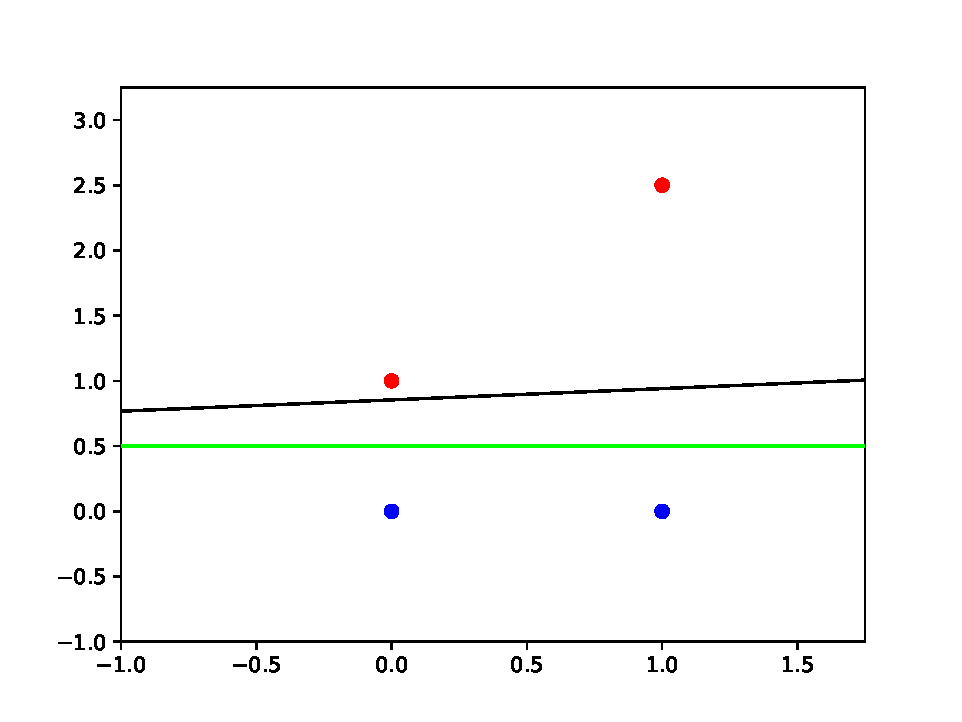
\includegraphics[scale=0.6]{SVMS.pdf}
	\end{center}
	\caption{Vergleich SVM und LS-SVM: In grün eingezeichnet ist die Trennebene der SVM, in schwarz die Trennebene der LS-SVM.}
	\label{fig:SVMS}
\end{figure}

In \autoref{fig:SVMS} wird der Unterschied zwischen den beiden Vorgehensweisen deutlich. Die grüne Linie markiert dabei die Trennebene der SVM und ist in diesem Beispiel sehr einfach nachzuvollziehen. Der Margin soll maximal werden, was bedeutet, dass die drei unten gelegenen Punkte die Support Vektoren bilden und die Ränder des Margin und dessen Breite definieren.\\
Die schwarze Linie ist die Trennebene der LS-SVM und verdeutlicht den Einfluss des oberen roten Punkts auf die Hyperebene. Würden noch weitere Punkte in die rote Klasse hinzugefügt, welche weit entfernt von der blauen Klasse liegen, so würde die Trennebene weiter nach oben und eventuell über den Punkt \(\left(0,1\right)\) hinausgeschoben, so dass dieser dann fehlerhaft klassifiziert wird.\\ 
Für weitere Theorie zur LS-SVM wird auf \cite{LS-SVM_b} verwiesen.